\documentclass{../source/Experiment}

\major{信息工程}
\name{姚桂涛}
\title{形态学和其他集合运算}
\stuid{3190105597}
\college{信息与电子工程学院}
\date{\today}
\lab{}
\course{数字图像处理}
\instructor{李东晓}
\grades{}
\expname{形态学和其他集合运算}
\exptype{设计验证}
\partner{}
\begin{document}
    \makecover
    \section{实验任务}

        本次选择的是PROJECT-10-02题目。

        \begin{enumerate}
            \item 编写一个程序实现基本全局阈值处理,输出应该为一个二值图像。
            \item 下载图10.38(a),进行全局阈值处理,其结果应该与书上的一样。
        \end{enumerate}

    \section{算法设计}
        算法实现如下:

        \begin{enumerate}
            \item 为全局阈值T选择一个初始估计值,这里用了图像的平均灰度值作为初值。
            \item 利用T分割图像,产生两组像素:G1由灰度值大于T的所有像素组成,G1由所有小于等于T的像素组成。
            \item 计算G1、G2的平均灰度值m1、m2。
            \item 得到新的阈值$\displaystyle T_{new} = \frac{1}{2}(m1+m2)$
            \item 重复步骤2到步骤4,直到T与T\_new的差值小于一个预定的值。
        \end{enumerate}


    \section{代码实现}
        本次实验编程语言选择的是Matlab。

        \lstinputlisting[
            language  =   matlab
            ]{第五次/lab_new.m}

    \section{实验结果}
        实验结果如下:

        \begin{figure}[H]
            \centering
            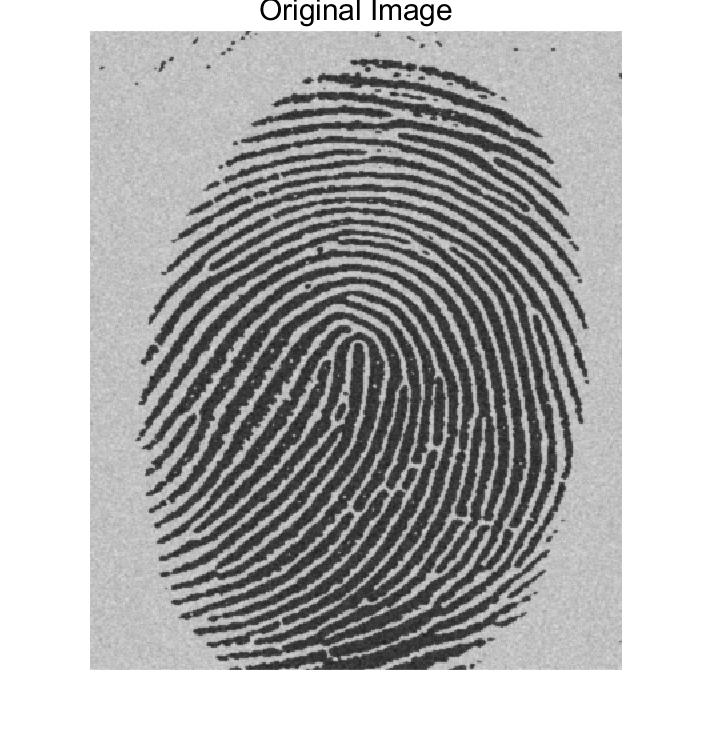
\includegraphics[width = 0.4\textwidth]{第五次/lab5-1.jpg}
            \caption{原始图像}
        \end{figure}

        \begin{figure}[H]
            \centering
            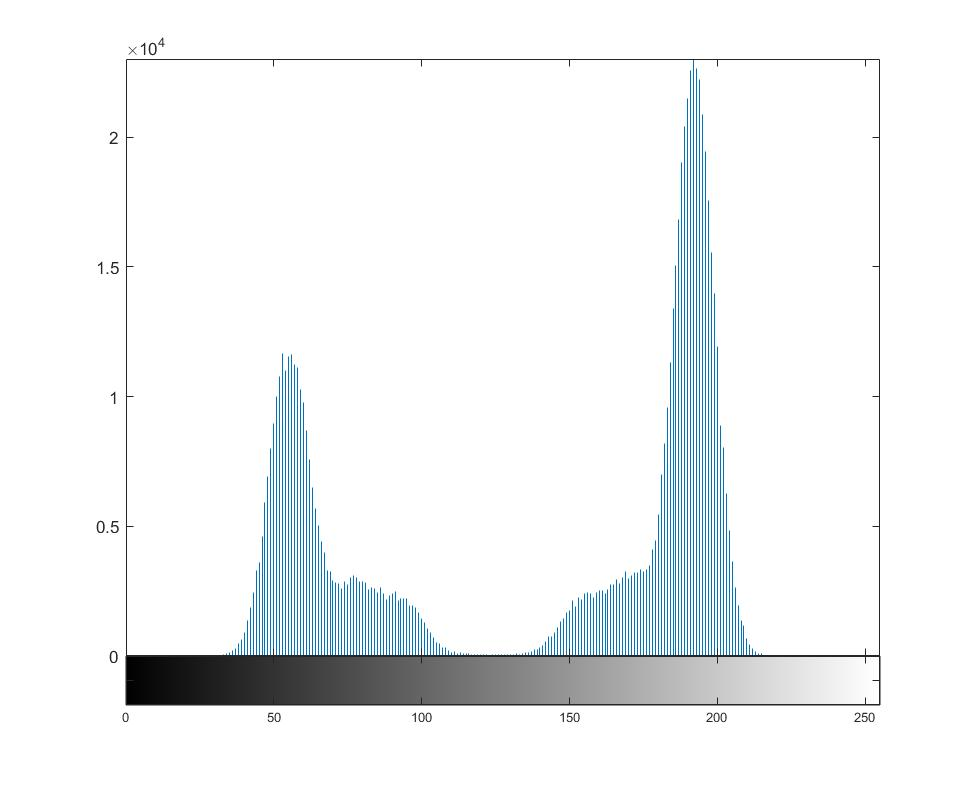
\includegraphics[width = 0.5\textwidth]{第五次/lab5-2.jpg}
            \caption{原始图像直方图}
        \end{figure}

        \begin{figure}[H]
            \centering
            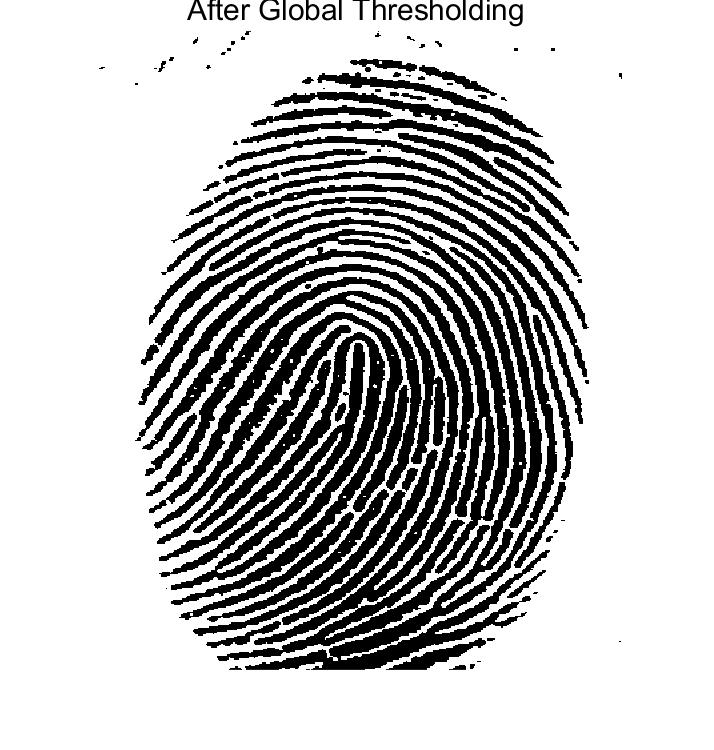
\includegraphics[width = 0.4\textwidth]{第五次/lab5-3.jpg}
            \caption{全局阈值处理后的图像}
        \end{figure}


    \section{总结}
    本次实验主要是通过Matlab编程语言实现了课程中所讲过的全局阈值处理。

    实验还是比较简单,但是基本的全局阈值处理对原始图像的要求高,需要原始图像的直方图有明显的波谷。

\end{document}



